\documentclass[12pt,a4paper]{article}
\usepackage[UTF8]{ctex}     %先引入ctex
\usepackage[utf8]{inputenc} %再引入inputenc
\usepackage{graphicx}
\usepackage{geometry}
\usepackage{xcolor}
% \usepackage{lazylatex}
\usepackage{amsmath}
\usepackage{enumerate}
\usepackage{caption}
\usepackage{listings}
\captionsetup[lstlisting]{labelfont=bf,justification=justified}

\usepackage{tikz}
\usepackage{pgfplots}
\pgfplotsset{compat=1.17}
\usepackage{appendix}

\graphicspath{{img/}}
% 边距
\geometry{left=2.0cm,right=2.0cm,top=2.0cm,bottom=3.0cm}
% 大题
\newenvironment{problems}{\begin{list}{}{\renewcommand{\makelabel}[1]{\textbf{##1}\hfil}}}{\end{list}}
% 小题
\newenvironment{steps}{\begin{list}{}{\renewcommand{\makelabel}[1]{##1.\hfil}}}{\end{list}}
% 答
\providecommand{\ans}{\textbf{答}:~}
% 解
\providecommand{\sol}{\textbf{解}.~}

\usepackage[colorlinks,linkcolor=blue]{hyperref}
\usepackage{bookmark}
\providecommand{\code}[2]{\lstinputlisting[language=#2,caption=\href{run:#1}{\ttfamily #1}]{#1}}
\providecommand{\img}[1]{\includegraphics[width=0.88\textwidth]{#1}}

% listings
\definecolor{grey}{rgb}{0.8,0.8,0.8}
\definecolor{darkgreen}{rgb}{0,0.3,0}
\definecolor{darkblue}{rgb}{0,0,0.3}
\lstset{%
    % numbers=left, %行号
    % numberstyle=\tiny\color{grey},
    showstringspaces=false,
    showspaces=false,%
    tabsize=4,%
    frame=shadowbox,%
    basicstyle={\ttfamily\scriptsize},%
    keywordstyle=\color{blue!80!black}\bfseries,%
    identifierstyle=,%
    commentstyle=\color{green!50!blue}\itshape,%
    stringstyle=\color{green!50!black},%
    rulesepcolor=\color{gray!20!white},
    breaklines,
    columns=flexible,
    extendedchars=false,
    %mathescape=true,
    language=c,
}

\begin{document}
\title{\normalsize \underline{操作系统(D)}\\\LARGE 项目 7}
\author{李子龙 518070910095}
\date{\today}
\maketitle

\textbf{连续内存分配}
\begin{problems}
    \item[一] \textbf{主框架}
    
    \includegraphics[width=0.88\textwidth]{input.png}

    这里采用一个 \texttt{alloc} 的结构存储进程内存信息:起始、大小和进程名、下一个进程:
    \begin{lstlisting}
#define MAXLINE 30
int MAX;

struct alloc
{
    int start;
    int size;
    char process[MAXLINE];
    struct alloc* next;
};
    \end{lstlisting}
    采用一个单链表存储内存信息,定义空间起始位置:
    \begin{lstlisting}
// List
struct alloc* space_head;
    \end{lstlisting}
    
    获取内存大小:
    \begin{lstlisting}
int main(int argc, char* argv[]){
    if(argc==1){
        fprintf(stderr, "Please assign the initial amount of memory.\n");
        return -1;
    }
    MAX = atoi(argv[1]);
    \end{lstlisting}

    分配初始内存块:
    \begin{lstlisting}
    space_head = (struct alloc*) malloc(sizeof(struct alloc));
    space_head->start = 0;
    space_head->size = MAX;
    strcpy(space_head->process,"Unused");
    space_head->next = NULL;
    \end{lstlisting}

    获取命令:
    \begin{lstlisting}
    char command[MAXLINE];
    do{
        fprintf(stdout, "allocator> ");
        fscanf(stdin, "%s", command);
        if(strcmp(command,"RQ")==0){
            char process[MAXLINE];
            int size;
            char flag[2];

            fscanf(stdin, "%s", process);
            fscanf(stdin, "%d", &size);
            fscanf(stdin, "%s", flag);

            if(request(process, size, flag))
                fprintf(stderr, "No sufficient memory!\n");
            
        } else if (strcmp(command,"RL")==0){
            char process[MAXLINE];
            fscanf(stdin, "%s", process);

            if(release(process))
                fprintf(stderr, "No such process to be released!\n");

        } else if (strcmp(command,"C")==0)
            compat();
        else if (strcmp(command,"STAT")==0) 
            status();
    } while(strcmp(command,"X")!=0);
}
    \end{lstlisting}

    \item[二] \textbf{状态}
    \begin{lstlisting}
void status() {
    struct alloc* tmp = space_head;
    while(tmp){
        char process_name[MAXLINE];
        if(strcmp(tmp->process,"Unused")==0) strcpy(process_name,"Unused");
        else { 
            strcpy(process_name, "Process ");
            strcat(process_name, tmp->process);
        };
        fprintf(stdout,"Addresses [%d:%d] %s\n", tmp->start, tmp->start + tmp->size - 1, process_name);
        tmp = tmp->next;
    }
}
    \end{lstlisting} 

    \item[三] \textbf{分配内存}
    
    请求两个进程,一个需要产生碎片,另一个是正好分配。

    \includegraphics[width=0.88\textwidth]{RQ.png}

    通过 \texttt{flag} 定义分配内存的方式。
    \begin{lstlisting}
int request(char* process, int size, char* flag){
    struct alloc* tmp = space_head;
    struct alloc* select = NULL;
    int besthole;
    switch(flag[0]){
        //...
    }
    \end{lstlisting}
    如果没有选择出孔,则会返回错误指标,终止分配。

    \includegraphics[width=0.88\textwidth]{RQN.png}

    \begin{lstlisting}
    if(!select) return 1;
    \end{lstlisting}
    如果选择出了孔,如果这个孔的大小比所需要的内存大,则会产生内部碎片。
    
    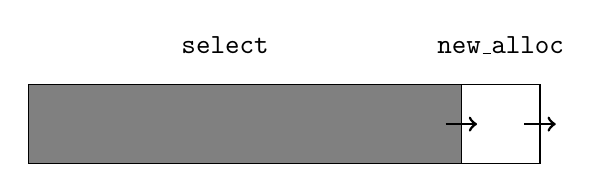
\begin{tikzpicture}

\draw  (-4.5,1.5) rectangle (2,0.5);
\draw [fill=gray] (-4.5,0.5) rectangle (1,1.5);
\node at (1.5,2) {\ttfamily new\_alloc};
\node at (-2,2) {\ttfamily select};
\draw[->,line width=1pt] (0.8,1) -- (1.2,1);
\draw[->,line width=1pt] (1.8,1) -- (2.2,1);
\end{tikzpicture}

    \begin{lstlisting}
    if(select->size > size){
        struct alloc* new_alloc = (struct alloc*) malloc(sizeof(struct alloc));
        new_alloc->start = select->start + size;
        new_alloc->size = select->size - size;
        strcpy(new_alloc->process,"Unused");
        new_alloc->next = select->next;
        
        select->size = size;
        strcpy(select->process, process);
        select->next = new_alloc;
    } 
    \end{lstlisting}
    如果刚好,就直接赋予该空间该进程即可。
    \begin{lstlisting}
    else if (select->size == size){
        strcpy(select->process, process);
    }
    return 0;
}
    \end{lstlisting}
    
    不同的分配方式:
    \begin{description}
        \item[首次适应] 选择第一个满足分配空间的孔。
        
        \includegraphics[width=0.88\textwidth]{RQF.png}
        
        \begin{lstlisting}
            case 'F':
            // First-fit
            while(tmp){
                if(strcmp(tmp->process,"Unused")==0 && tmp->size >= size){
                    select = tmp;
                    break;
                }
                tmp = tmp -> next;
            }
            break;
        \end{lstlisting} 
        \item[最优适应] 遍历所有的孔,选择能够使得碎片大小最小的孔。
        
        \includegraphics[width=0.88\textwidth]{RQB.png}
         
        \begin{lstlisting}
            case 'B':
            // Best-fit
            besthole = MAX;
            while(tmp){
                if(strcmp(tmp->process,"Unused")==0 && tmp->size >= size && tmp->size - size < besthole){
                    select = tmp;
                    besthole = tmp->size - size;
                }
                tmp = tmp->next;
            }
            break;
        \end{lstlisting} 
        \item[最差适应] 遍历所有的孔,选择能够使碎片大小最大的孔。
        
        \includegraphics[width=0.88\textwidth]{RQW.png}
        
        \begin{lstlisting}
            case 'W':
            // Worst-fit
            besthole = -1;
            while(tmp){
                if(strcmp(tmp->process,"Unused")==0 && tmp->size >= size && tmp->size - size > besthole){
                    select = tmp;
                    besthole = tmp->size - size;
                }
                tmp = tmp -> next;
            }
            break;
        \end{lstlisting} 
    \end{description}
    
    \item[四] \textbf{释放内存}
    
    先单独考虑释放的进程是开头的进程。
    \begin{lstlisting}
int release(char *process){
    struct alloc* tmp = space_head;
    if(strcmp(tmp->process, process)==0){

        // X -> O
        // X X -> O X
        // X O -> O
    \end{lstlisting}
    对于开头进程的释放有三种情况:
    \begin{enumerate}
        \item 如果开始的进程后面没有进程了,就直接置零。
        
        \includegraphics[width=0.88\textwidth]{RL11.png}

        \begin{lstlisting}
        int after = (tmp->next ? strcmp(tmp->next->process,"Unused") == 0 : 0);
        \end{lstlisting}
        \item 如果开头的进程后面是碎片,就需要将释放后的空间与该碎片合并。
        
        \includegraphics[width=0.88\textwidth]{RL12.png}

        \begin{lstlisting}
        if (after){
            space_head = tmp->next;
            space_head->start -= tmp->size;
            space_head->size += tmp->size;
        }
        \end{lstlisting}
        \item 如果开头的进程后面是进程,就直接置零。
        
        \includegraphics[width=0.88\textwidth]{RL13.png}

        \begin{lstlisting}
            else {
                strcpy(space_head->process, "Unused");
            }
            return 0;
        }
        \end{lstlisting}
    \end{enumerate}

    类似的,对于中间进程的释放,需要分成四种情况:
    \begin{lstlisting}
        while(tmp->next){
            if(strcmp(tmp->next->process,process)==0){
                struct alloc* del = tmp->next;
    
                // O X O -> O
                // X X O -> X O
                // O X X -> O X
                // X X X -> X O X

                int before = strcmp(tmp->process,"Unused") == 0;
                int after = (tmp->next->next ? strcmp(tmp->next->next->process,"Unused") == 0 : 0);
    \end{lstlisting}
    \begin{enumerate}
        \item 前后都为孔,就需要将三孔合一。
        
        \includegraphics[width=0.88\textwidth]{RL21.png}

        \begin{lstlisting}
            if(before && after){
                tmp->size += del->size + tmp->next->next->size;
                tmp->next = tmp->next->next;
            }
        \end{lstlisting}
        \item 后为孔,后两个合一。
        \begin{lstlisting}
            else if (after){
                tmp->next->next->start -= del->size;
                tmp->next->next->size += del->size;
                tmp->next = tmp->next->next;
            }
        \end{lstlisting}
        \item 前为孔,前两个合一。
        \begin{lstlisting}
            else if (before){
                tmp->size += del->size;
                tmp->next = tmp->next->next;
            }
        \end{lstlisting}
        \item 都不为孔,直接置零。
        \begin{lstlisting}
            else {
                strcpy(del->process,"Unused");
            }
        \end{lstlisting}
    \end{enumerate}
    最后移动指标。如果遍历到最后都没有找到,就会返回未找到。
    
    \includegraphics[width=0.88\textwidth]{RL22.png}
        \begin{lstlisting}
            return 0;
        }
        tmp = tmp->next;
    }
    return 1;
}
    \end{lstlisting}
    \item[五] \textbf{紧缩}
    
    首先寻找尾部,并存储遍历的块次数 \texttt{count}。
    \begin{lstlisting}
void compat() {

    struct alloc* tail = space_head;
    int count = 1;
    while(tail->next){
        tail = tail->next;
        ++count;
    }

    // Move to tail
    // O O X X X -> O X X X O -> X X X O O
    // O X X X X -> X X X X O
    // X O X O X -> X X O X O -> X X X O O

    \end{lstlisting} 

    紧缩共分两步:移动碎片到尾部、碎片合一。
    
    对于移动碎片,分两种情形:
    \begin{enumerate}
        \item 头部是碎片。需要移动空间头 \texttt{space\_head} 标记的位置,并遍历到尾部将所有的块开始位置前移,再将碎片挂载在尾部。
        
        \includegraphics[width=0.88\textwidth]{C1.png}        

        \begin{lstlisting}
            struct alloc* tmp = space_head;
            while (tmp->next && strcmp(tmp->process,"Unused")==0){
                space_head = tmp->next;
        
                struct alloc* ch_tmp = space_head;
                while(ch_tmp){
                    ch_tmp->start -= tmp->size;
                    ch_tmp = ch_tmp->next;
                }
                
                tmp->next = tail->next;
                tmp->start = tail->start + tail->size;
                tail->next = tmp;
                tail = tmp;
                tmp = space_head;
                --count;
                if(!count) break;
            }
        \end{lstlisting}
        \item 中间某处是碎片。需要多计算一次移动次数,因为移动了一个指针,并移动了一个块。
        
        \includegraphics[width=0.88\textwidth]{C2.png}

        \begin{lstlisting}
    while(count) {
        if(!tmp->next) break;
        if(tmp->next->next && strcmp(tmp->next->process,"Unused")==0){
            struct alloc* mover = tmp->next;
            tmp->next = tmp->next->next;

            struct alloc* ch_tmp = tmp->next;
            while(ch_tmp){
                ch_tmp->start -= mover->size;
                ch_tmp = ch_tmp->next;
            }
            
            mover->next = tail->next;
            mover->start = tail->start + tail->size;
            tail->next = mover;
            tail = mover;
            --count;
        }
        tmp = tmp->next;
        --count;
    }
    \end{lstlisting}
    \end{enumerate}

    最后将所有的碎片紧缩为一个空余空间。
    \begin{lstlisting}
    // Compat the space
    while(tmp && tmp->next){
        tmp->size += tmp->next->size;
        tmp->next = tmp->next->next;
    }
}
    \end{lstlisting}

\end{problems}

\begin{appendices}
    \section{全部代码}
    \code{src/Makefile}{}
    \code{src/cma.c}{c}
\end{appendices}

\end{document}